\documentclass{beamerthemeMono}

% specify some optional logos
\graphicspath{{figures/}}
%\pgfdeclareimage[height=1.45cm]{mainlogo}{figures/logo}
\pgfdeclareimage[height=1.4cm]{mainlogo}{figures/logo.pdf}
% placed in the lower left/right corner if the \pgfuseimage{minilogo}
% command is uncommented in the \institute command below.
\pgfdeclareimage[height=1cm]{minilogo}{figures/logo.pdf}
\logo{\pgfuseimage{minilogo}}

\AtBeginSection[] {
  \begin{frame}
    \frametitle{目录} 
    {\tableofcontents[%
      currentsection, % causes all sections but the current to be shown in a semi-transparent way.
%     currentsubsection, % causes all subsections but the current subsection in the current section to ...
      hideallsubsections, % causes all subsections to be hidden.
%     hideothersubsections, % causes the subsections of sections other than the current one to be hidden.
%      part=2 % part number causes the table of contents of part part number to be shown
%     pausesections, % causes a \pause command to be issued before each section. This is useful if you
%     pausesubsections, %  causes a \pause command to be issued before each subsection.
      %sections={<1-3|handout:0>} %{ overlay specification },
      ]}
   \end{frame}}

\makeatletter
\AtBeginPart{%
  \beamer@tocsectionnumber=0\relax
  \setcounter{section}{0}
  \frame[plain]{\partpage}%
}
\makeatother

% \AtBeginPart{
%      \begin{frame}[plain]
%          \partpage
%      \end{frame}}

% \AtBeginSubsection[]                            % 在每个子段落之前
% {
%   \frame{                                         % handout:0 表示只在手稿中出现
%     \frametitle{目录} \small
%     \tableofcontents[
%       currentsection,
%       currentsubsection,
%       subsectionstyle=show/shaded/hide]
%   }
% }
%%%%%%%%%%%%%%%%%%%%%%%%%%%%%%%%%%%%%%%%%%%%%%%%%%%%%%%%%%%%
%%%%%%%%%%%%%%%%%%%%%%%%%%%%%%%%%%%%%%%%%%%%%%%%%%%%%%%%%%%%
          % 文档开始
%%%%%%%%%%%%%%%%%%%%%%%%%%%%%%%%%%%%%%%%%%%%%%%%%%%%%%%%%%%%
%%%%%%%%%%%%%%%%%%%%%%%%%%%%%%%%%%%%%%%%%%%%%%%%%%%%%%%%%%%%

\begin{document}

\title[交通规划行业中的数据应用现状及思考]% optional, use only with long paper titles
{\heiti \xiaoerhao 交通规划行业中的数据应用现状及思考}


\author[邹海翔] % optional, use only with lots of authors
{\xiaosihao 邹海翔}
\date{\xiaosihao 2019年2月}
 % - Give the names in the same order as they appear in the paper.  -
 % Use the \inst{?} command only if the authors have different
 % affiliation. See the beamer manual for an example


\institute[综合交通所] % optional - is placed in the bottom of the sidebar on every slide
{%
   \xiaosihao 综合交通所
   % there must be an empty line above this line - otherwise some
   % unwanted space is added
   % between the university and the country (I do not know why)
}

 % \date{\today}
\titlegraphic{\pgfuseimage{mainlogo}} %insert a company or department logo


 % the titlepage the plain option removes the sidebar and header from
 % the title page
\begin{frame}[plain]
  \titlepage
\end{frame}
%%%%%%%%%%%%%%%%


\begin{frame}{大纲}{}
   {\tableofcontents[hideallsubsections]}
\end{frame}

%%%%%%%%%%%%%%%%%%%%%%%%%%%%%%%%%%%%%%%%%%%%%%%%%%%%%%%%%%%%

%%%%%%%%%%%%%%%%%%%%%%%%%%%%%%%%%%%%%%%%%%%%%%%%%%%%%%%%%%%%
\section{大数据时代下的交通规划}

\subsection{交通规划业务}

\begin{frame}[t]{\subsecname}
\begin{itemize}
\item 交通规划是城市规划的重要组成部分,主要目的是\emphText{建设和改善城市交通系统},从城市规模、用地布局、道路组织等
源头出发,提出解决城市交通问题的对策和具体方案
\item 交通规划是一项\emphText{综合性业务},除了交通以外,还涉及城市空间、人口、土地利用、公共政策等多方面的因素
\item 交通规划的成果主要是\emphText{各层次的规划编制方案},用于辅助城市管理者的决策,并指导落实最终的建设实施
\end{itemize}

\begin{columns}
  \begin{column}{.4\textwidth}
    \begin{figure}\flushright
      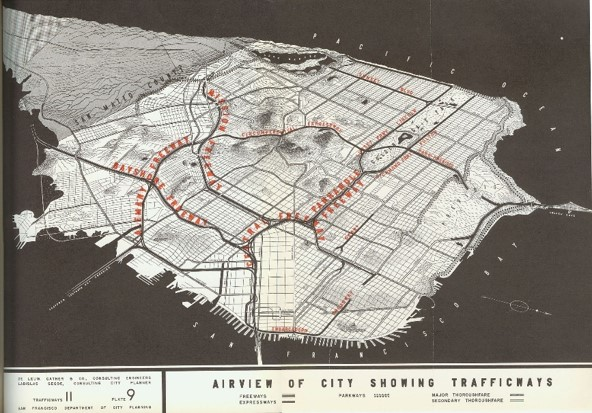
\includegraphics[height=0.3\textheight]{chp01_旧金山.jpg}
      \caption{1948年旧金山路网规划图}
    \end{figure}
  \end{column}
  \begin{column}{.6\textwidth}
    \begin{figure}\flushleft
      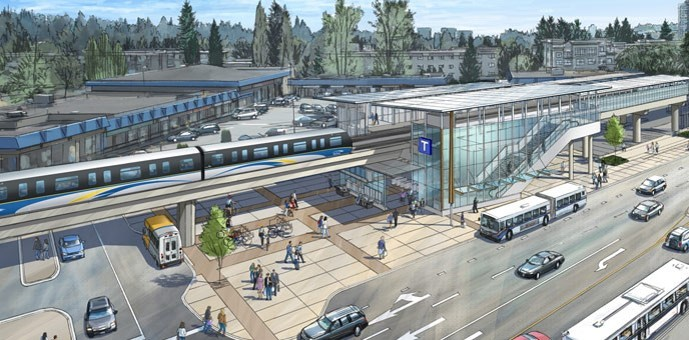
\includegraphics[height=0.3\textheight]{chp01_交通设计.jpg}
      \caption{城市公交站点交通设计图}
    \end{figure}
  \end{column}
\end{columns}
\end{frame}

\begin{frame}[t]{\subsecname}
\begin{itemize}
\item \emphText{交通调查}是交通规划业务最主要的数据来源,并以此为依据建立分析模型推断规划方案
\item 国内一般\emphText{5--10年}进行一次城市居民出行调查,每次调查的时间长达数月甚至一年
\end{itemize}

\begin{figure}
  \centering
  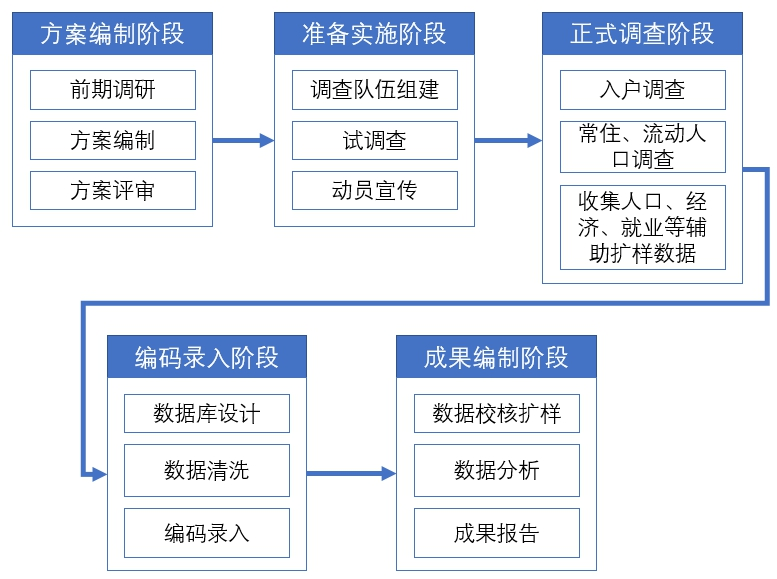
\includegraphics[width=0.65\textwidth]{chp01_交通调查.jpg}
  \caption{交通调查的一般流程}
\end{figure}
\end{frame}

\subsection{什么是大数据}

\begin{frame}[t]{\subsecname}
\begin{goodbox}{IBM公司对大数据的定义}
\begin{enumerate}\footnotesize
    \item Volume:海量的数据规模
    \item Velocity:快速的数据流转和动态的数据体系
    \item Variety:多样的数据类型
    \item Value:巨大的数据价值
    \item Veracity:数据的准确性和可信赖度
\end{enumerate}
\end{goodbox}

\begin{figure}
\begin{columns}
  \begin{column}{.5\textwidth}
      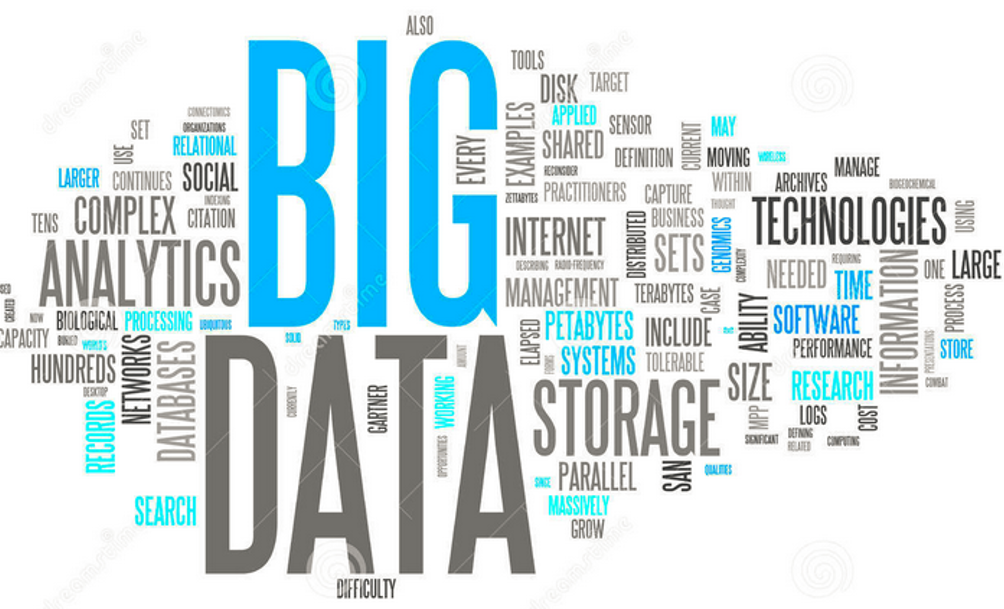
\includegraphics[height=0.35\textheight]{chp01_文字云.png}
  \end{column}
  \begin{column}{.5\textwidth}
      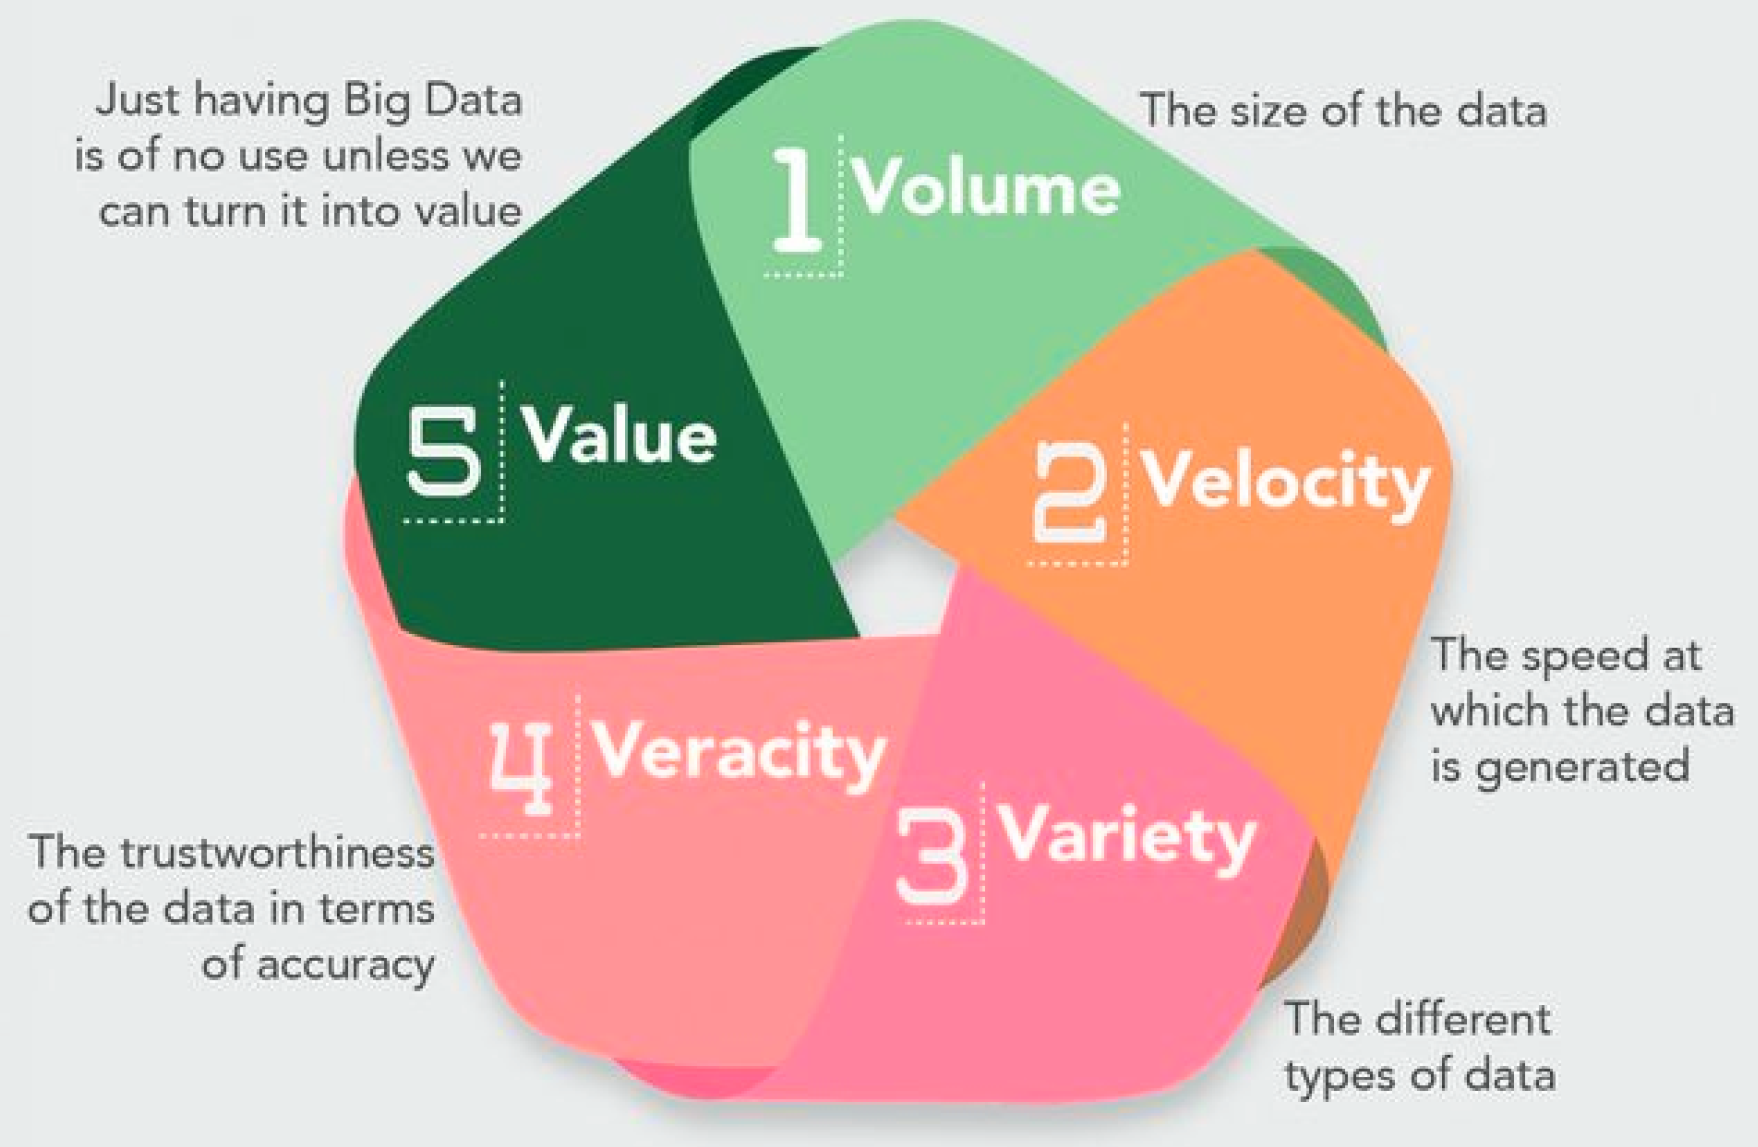
\includegraphics[height=0.35\textheight]{chp01_5V.png}
  \end{column}
\end{columns}
\caption{大数据的5V定义}
\end{figure}
\end{frame}

\begin{frame}[t]{\subsecname}
\begin{itemize}
\item<1-> 与传统数据相比,不仅体现在数据量巨大,更重要的是可以覆盖业务的近乎全部数据
\item<2-> 数据爆炸时代的必然产物
\item<3-> 商业公司进行的一场成功的营销 
\end{itemize}

\begin{overlayarea}{\textwidth}{\textheight}
  \begin{onlyenv}<4>
     \begin{columns}
       \begin{column}{.3\textwidth}
       \begin{figure}
         \centering 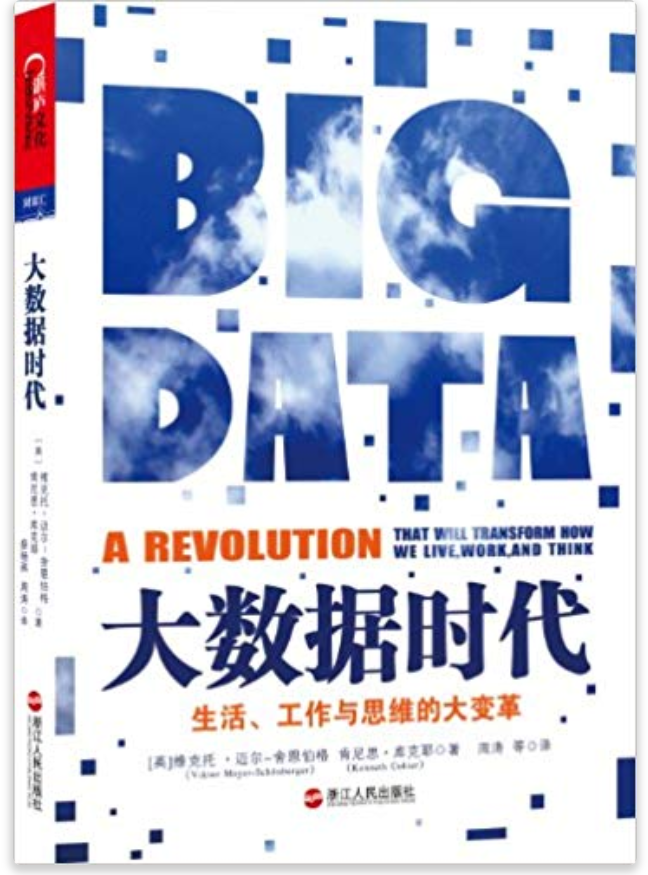
\includegraphics[width=\columnwidth]{chp01_bigdatabook.png}
       \end{figure}
       \end{column}
       \begin{column}{.7\textwidth}
      \begin{ornamentblock}
          \hspace*{2em}大数据是一场思维的颠覆:放弃对因果关系(为什么)的渴求,
而取而代之关注相关关系(是什么)。\\
          \rightline{\textemdash 维克托$\cdot$迈尔$\cdot$舍恩伯格}
      \end{ornamentblock}
       \end{column}
     \end{columns}
  \end{onlyenv}
\end{overlayarea}
\end{frame}

\subsection{大数据对规划编制的意义}

\begin{frame}[t]{\subsecname}
\begin{itemize}
\item<1-> 外部条件与时代背景
\pause
\begin{commonbox}{技术进步} 
随着计算机技术的发展,尤其是云计算和人工智能技术的进步,使得数据获取变得容易了许多,而且处理和分析的能力越来越强
\end{commonbox}
\pause 
\begin{commonbox}{经济转型} 
当前中国的经济正处于重要的转型时期,经济的发展模式、发展要素、发展路径等等都亟需转变,以适应现在的大环境
\end{commonbox}
\pause
\begin{commonbox}{社会转型} 
虽然我们的经济实现了快速发展,但社会矛盾出现越来越尖锐化的趋势
\end{commonbox}
% \begin{commonbox}{规划转型} \footnotesize
% 当前的城市规划也面临着从粗放向集约转型、从城市向区域转型、从外观向内在转型等
% \end{commonbox}
\end{itemize}
\end{frame}

\begin{frame}[t]{\subsecname}
\begin{itemize}
\item 传统城市空间规划面临方法转型
\end{itemize}

\begin{commonbox}{规划转型} 
\begin{itemize} 
\item 传统时空间概念被重新定义,以空间研究和布局为核心内容的城市空间规划
面临着研究范式的转型和规划编制方法上的革新
\item 随着国内城市化进程的发展,规划面临的更多是城市的存量式发展,由粗放向集约进行转型,
对规划的精细化、定量化管理提出了要求
\end{itemize}
\end{commonbox}
\begin{figure}
  \centering
  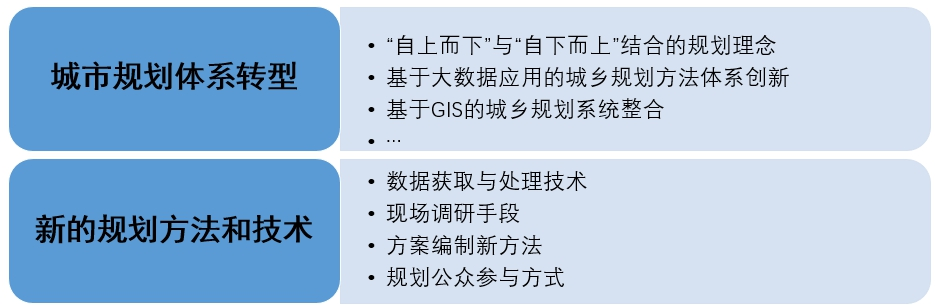
\includegraphics[width=0.85\textwidth]{chp01_规划转型.jpg}
  \caption{南京大学规划专业试行的学科教学改革方案}
\end{figure}
\end{frame}

\begin{frame}[t]{\subsecname}
\begin{itemize}
\item 大数据提供了认识和分析城市问题新的思维和技术方法
\item 大数据时代到来,可以让我们更清楚地了解和观察城市的发展、变化过程,同时也使得规划过程变得透明可控;
\item 大数据技术强化了对规划过程的重视和科学化,尤其是对规划调研、空间分析、公共参与与空间协调规划、
空间预测和可视化等过程的科学把握,有助于推动规划过程的科学化
\end{itemize}
\begin{figure}
  \centering
  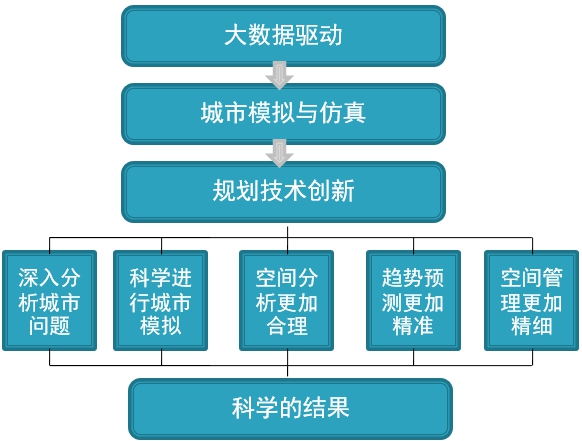
\includegraphics[width=0.55\textwidth]{chp01_数据驱动的城市规划.jpg}
  \caption{大数据驱动的规划决策评估架构}
\end{figure}
\end{frame}

%%%%%%%%%%%%%%%%%%%%%%%%%%%%%%%%%%%%%%%%%%%%%%%%%%%%%%%%%%%%

%%%%%%%%%%%%%%%%%%%%%%%%%%%%%%%%%%%%%%%%%%%%%%%%%%%%%%%%%%%%
\section{数据``菜谱''}

\subsection{菜谱}
\begin{frame}{\subsecname}
\begin{itemize}
\item<2-> 静态调查数据
   \begin{enumerate}
     \item 居民出行调查数据
     \item 跨界调查数据
   \end{enumerate}
\item<3-> 动态大数据
   \begin{enumerate}
       \item 公交刷卡数据
       \item 车辆GPS数据
       \item 车牌识别数据
       \item 手机数据
   \end{enumerate}
\item<4-> 地理信息数据
   \begin{enumerate}
     \item 土地利用数据
     \item 人口岗位数据
     \item 建筑物数据
  \end{enumerate}
\item<5-> 互联网开放数据
   \begin{enumerate}
     \item 地图
     \item 遥感影像
     \item 交通出行
  \end{enumerate}
\end{itemize}
\end{frame}
\end{frame}

\subsection{居民出行调查数据}

\begin{frame}[t]{\subsecname}
\begin{itemize}
\item<2-> 2005、2010、2016三次居民出行调查数据
\item<3-> 最终数据成果是\emphText{户表、人表和出行表}共三张表
\end{itemize}

\begin{overlayarea}{\textwidth}{\textheight}
  \begin{onlyenv}<2>
\begin{figure}
  \centering
  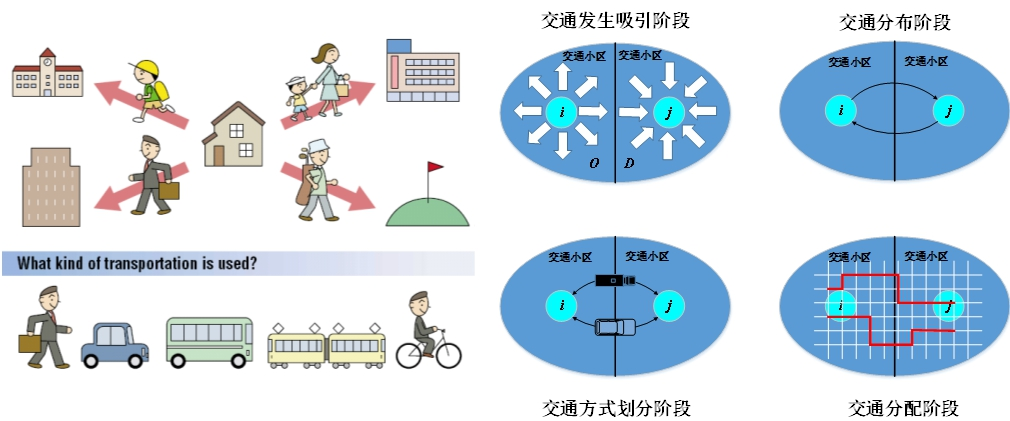
\includegraphics[width=\textwidth]{chp01_居民出行调查.jpg}
  \caption{以家庭为单位,调查家庭成员出行次数、出行目的、交通方式和目的地}
\end{figure}
  \end{onlyenv}

\begin{onlyenv}<3>
  \begin{table} \centering \footnotesize
    \begin{tabular}{|>{\centering\arraybackslash} m{0.15\columnwidth}|m{0.7\columnwidth}|}
      \toprule
      \rowcolor{LightCyan}
      \multicolumn{1}{|c|}{\textbf{主要字段}} & \multicolumn{1}{c|}{\textbf{说明}} \\\hline
      户ID & 唯一值\\\hline
      回答时间 & 填写问卷的时间\\\hline
      建筑物位置 & 被访问者居住地,经纬度坐标\\\hline
      户类型 & 家庭户:1;集体户:2\\\hline
      居住人数 & 分为$\geq{4}$岁人数和$<4$岁人数\\\hline
      家庭年收入 & $\leq{4}$万:1;10-20万:2;20-30万:3;30-50万:4;$\geq{50}$万:5\\\hline
      住房来源 & 租赁廉租房、租赁城中村、租赁其他住房、自建房、购买商品房、购买福利房或保障房、集体宿舍\\\hline
      拥车情况 & 是否拥有小汽车?家庭拥有几辆小汽车?\\\hline
      \bottomrule
    \end{tabular}
    \caption{户表}
  \end{table}
\end{onlyenv}

\begin{onlyenv}<4>
  \begin{table} \centering \footnotesize
    \begin{tabular}{|>{\centering\arraybackslash} m{0.15\columnwidth}|m{0.7\columnwidth}|}
      \toprule
      \rowcolor{LightCyan}
      \multicolumn{1}{|c|}{\textbf{主要字段}} & \multicolumn{1}{c|}{\textbf{说明}} \\\hline
      人ID & 与户ID对应\\\hline
      年龄 & \\\hline
      性别 & \\\hline
      户口登记情况 & 本市户籍:1;非本市户籍:2。其中,非本市户籍中是否居住6个月以上\\\hline
      文化程度 & 分为9个选项\\\hline
      职业 & 分为9个选项\\\hline
      所属行业 & 参考经济普查问卷,分为18个选项\\\hline
      工作地或学校地址 & \\\hline
      \bottomrule
    \end{tabular}
    \caption{人表}
  \end{table}
\end{onlyenv}

\begin{onlyenv}<5>
  \begin{table} \centering \footnotesize
    \begin{tabular}{|>{\centering\arraybackslash} m{0.4\columnwidth}|m{0.5\columnwidth}|}
      \toprule
      \rowcolor{LightCyan}
      \multicolumn{1}{|c|}{\textbf{主要字段}} & \multicolumn{1}{c|}{\textbf{说明}} \\\hline
      出行ID & 与人ID对应\\\hline
      出行和换乘方式 & 公交、小汽车、地铁等共12类\\\hline
      出行目的 & 上班、上学、公务等10类\\\hline
      出发时间 & \\\hline
      出发地点 & 详细地址及经纬度\\\hline
      到达时间 & \\\hline
      到达地点 & 详细地址及经纬度\\\hline
      换乘站点 & \\\hline
      步行时间、候车时间、车内时间 & 公共交通出行 \\\hline
      \bottomrule
    \end{tabular}
    \caption{出行表}
  \end{table}
\end{onlyenv}
\end{overlayarea}
\end{frame}

\subsection{跨界调查数据}

\begin{frame}[t]{\subsecname}
\begin{itemize}
\item 从2013年开始,每两年开展一次跨界客流调查
\item 调查范围包括深圳和东莞、惠州的边界、深圳出境口岸和重要对外交通枢纽
\end{itemize}

\begin{overlayarea}{\textwidth}{\textheight}
  \begin{onlyenv}<2>
\begin{figure}
  \centering
  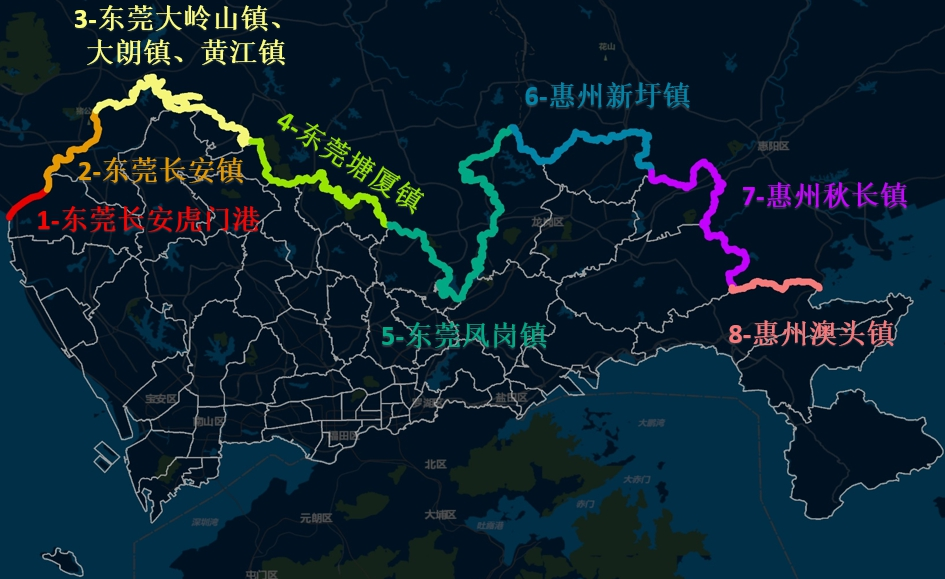
\includegraphics[width=0.85\textwidth]{chp02_境界线.jpg}
  \caption{深莞惠境界线}
\end{figure}
  \end{onlyenv}

  \begin{onlyenv}<3>
\begin{figure}
  \centering
  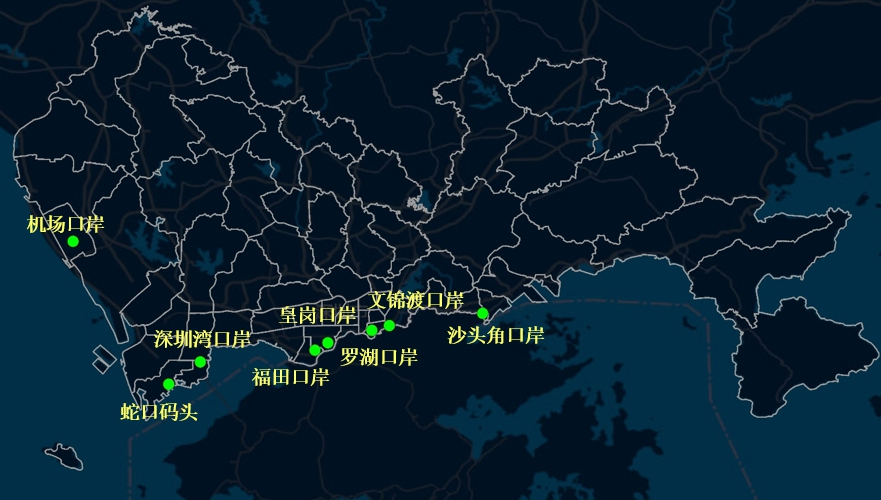
\includegraphics[width=0.85\textwidth]{chp02_口岸.jpg}
  \caption{深港口岸}
\end{figure}
  \end{onlyenv}

  \begin{onlyenv}<4>
\begin{figure}
  \centering
  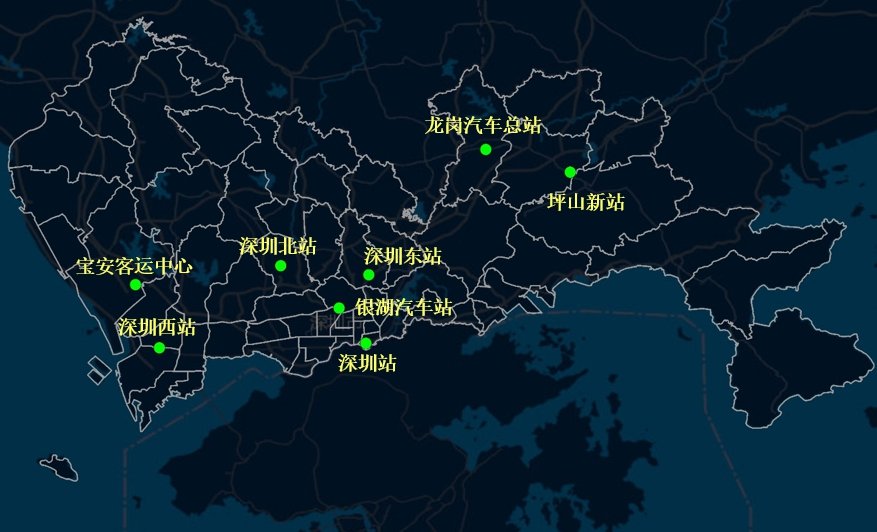
\includegraphics[width=0.8\textwidth]{chp02_交通枢纽.jpg}
  \caption{重要对外交通枢纽}
\end{figure}
  \end{onlyenv}
\end{overlayarea}
\end{frame}

\subsection{车辆GPS数据}

\begin{frame}[t]{\subsecname}
\begin{itemize}
\item<1-> 利用GPS卫星定位车辆,记录车辆位置、时间、方向、速度和状态等信息
\item<1-> 覆盖全部出租车、公交车、特种车以及部分货车,约10万辆
\item<2-> 从2013年开始收集,10-40秒回传一次数据,日均数据量约10GB左右,超过1亿条 
\end{itemize}

\begin{overlayarea}{\textwidth}{\textheight}
  \begin{onlyenv}<1>
\begin{figure}
  \centering
  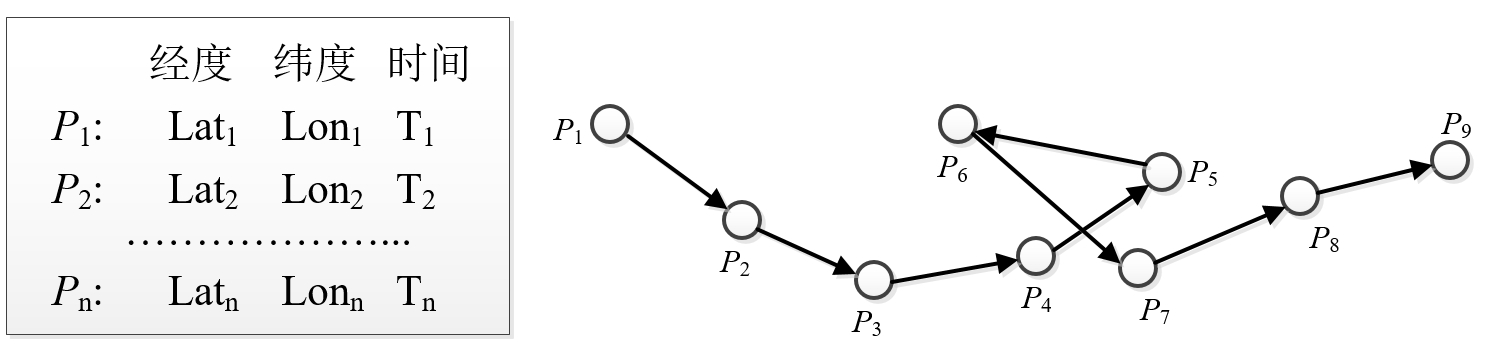
\includegraphics[width=\textwidth]{chp02_GPS示意图.jpg}
  \caption{GPS数据示意图}
\end{figure}
  \end{onlyenv}

\vspace{-10pt}
  \begin{onlyenv}<2>
\begin{figure}
  \centering
  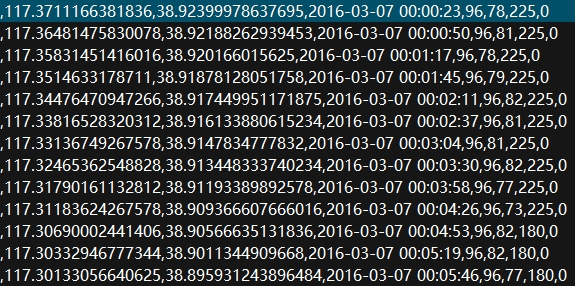
\includegraphics[width=0.85\textwidth]{chp02_GPS原始数据.jpg}
  \caption{GPS原始数据文件,每辆车存储一个文件}
\end{figure}
  \end{onlyenv}

\vspace{-5pt}
  \begin{onlyenv}<3>
\begin{figure}
  \centering
  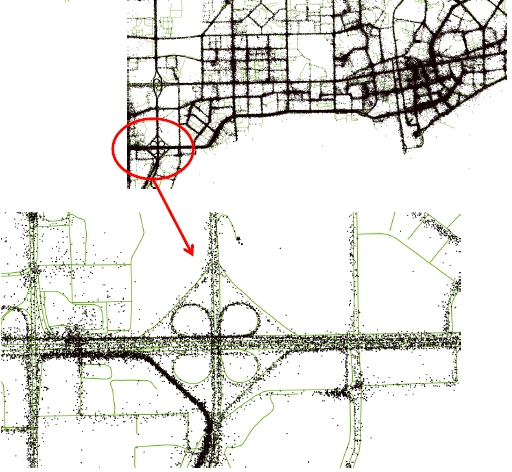
\includegraphics[width=0.5\textwidth]{chp02_空间上的GPS数据.jpg}
  \caption{空间中的GPS数据}
\end{figure}
  \end{onlyenv}
\end{overlayarea}
\end{frame}

\subsection{车牌识别数据}

\begin{frame}[t]{\subsecname}
\begin{itemize}
\item<1-> 通过车牌识别算法,从布设在道路上的拍摄视频中提取车牌
\item<2-> 全市目前有300多个检测点位
\item<2-> 从2014年开始收集,日均数据量是约2.5GB,超过1200万条 
\end{itemize}

%\begin{overlayarea}{\textwidth}{\textheight}

%\vspace{15pt}
\begin{onlyenv}<1>
\begin{figure} \centering
\begin{columns}[b]
  \begin{column}{.5\textwidth}
    \begin{figure}\flushright
      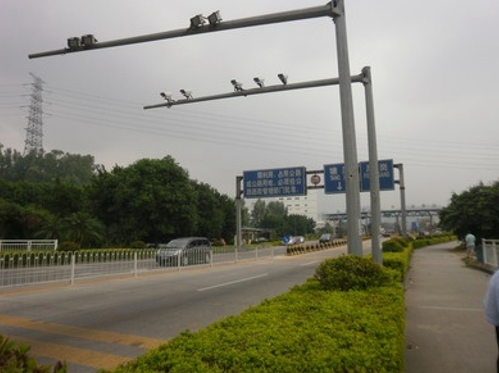
\includegraphics[height=0.35\textheight]{chp02_车牌识别01.jpg}
    \end{figure}
  \end{column}
  \begin{column}{.5\textwidth}
    \begin{figure}\flushleft
      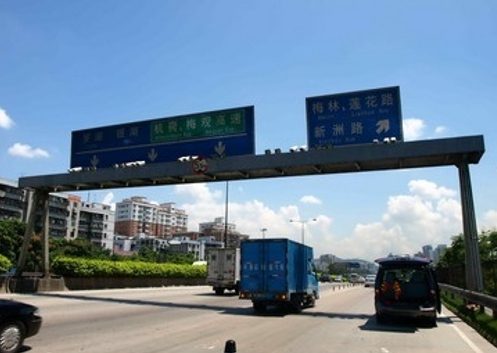
\includegraphics[height=0.35\textheight]{chp02_车牌识别02.jpg}
    \end{figure}
  \end{column}
\end{columns}
\caption{道路上的车辆拍摄设备} 
\end{figure}
\end{onlyenv}
%\end{overlayarea}

\end{frame}

%%%%%%%%%%%%%%%%%%%%%%%%%%%%%%%%%%%%%%%%%%%%%%%%%%%%%%%%%%%%

%%%%%%%%%%%%%%%%%%%%%%%%%%%%%%%%%%%%%%%%%%%%%%%%%%%%%%%%%%%%
\section{数据分析的``武器库''}

%%%%%%%%%%%%%%%%%%%%%%%%%%%%%%%%%%%%%%%%%%%%%%%%%%%%%%%%%%%%

%%%%%%%%%%%%%%%%%%%%%%%%%%%%%%%%%%%%%%%%%%%%%%%%%%%%%%%%%%%%
\section{数据在业务中的应用案例}

%%%%%%%%%%%%%%%%%%%%%%%%%%%%%%%%%%%%%%%%%%%%%%%%%%%%%%%%%%%%

%%%%%%%%%%%%%%%%%%%%%%%%%%%%%%%%%%%%%%%%%%%%%%%%%%%%%%%%%%%%
\section{再认识与展望}

%%%%%%%%%%%%%%%%%%%%%%%%%%%%%%%%%%%%%%%%%%%%%%%%%%%%%%%%%%%%

%%%%%%%%%%%%%%%%%%%%%%%%%%%%%%%%%%%%%%%%%%%%%%%%%%%%%%%%%%%%

%%%%%%%%%%%%%%%%%%%%%%%%%%%%%%%%%%%%%%%%%%%%%%%%%%%%%%%%%%%%%%%%%%%%%%%%%%%%
% 结束页
%%%%%%%%%%%%%%%%%%%%%%%%%%%%%%%%%%%%%%%%%%%%%%%%%%%%%%%%%%%%%%%%%%%%%%%%%%%%
\begin{frame}[plain,noframenumbering]%
  \finalpage{
    \begin{table} \Huge \centering
      \begin{tabular}{c}
        汇~报~结~束\\
        谢~谢!
      \end{tabular} \end{table}
    \titlegraphic{\pgfuseimage{mainlogo}}}
\end{frame}
\end{document}
%%% Local Variables:
%%% mode: latex
%%% TeX-master: t
%%% End:
